\section{Exercises}
\label{section:finiteStateMachines}
\graphicspath{ {./chapter07/FigHw} }

\begin{enumerate}
    \item A finite state machine has been implemented with four
        flip-flops, two inputs and three outputs.
        \begin{enumerate}
            \item What are the minimum and maximum number of states in the diagram?
                \begin{onlysolution}  \textbf{Solution} \itshape{
                        Since there are three flip flops we can have a maximum of 8 states.  The minimum
                        number of states is a bit tricky.  A practical answer is 5, because if you
                        had fewer states you would use fewer flip flops.  However, the question
                        asks for a minimum, in which case you could have 1 state.  Note, that a
                        1 state FSM would only generate a single output and hence would not be a
                        very interesting circuit.
                    }
                \end{onlysolution}
            \item What are the minimum and maximum number of transition arrows
                starting at a particular state?
                \begin{onlysolution}  \textbf{Solution} \itshape{
                        These values are the same.  Since there are two bits of input there are four
                        different inputs that can be applied at each state.  Thus, four arrows must
                        leave each state.
                    }
                \end{onlysolution}
            \item What are the minimum and maximum number of transition arrows
                ending in a particular state?
                \begin{onlysolution}  \textbf{Solution} \itshape{
                        In a typical design your systems will have a reset state, it normal for such
                        states to have NO input arcs.  You only visit them when the power is turned on.
                        This is the minimum number of arcs that can terminate at a state.  On the
                        other hand, I could image a machine where   transition arc points to a
                        particular state (not a very interesting FSM).  Hence all 32 arcs could point
                        to a single state.
                    }
                \end{onlysolution}
            \item What are the minimum and maximum number of different binary patterns
                that are displayed on the outputs?
                \begin{onlysolution}  \textbf{Solution} \itshape{
                        this is a tricky question, you need to determine which of the inputs and outputs
                        constrains the number of distinct patterns on the output.  You should consult
                        figure 7.1 for some guidance.  There are three bits of output which have the possibility
                        of generating 8 different outputs.  There are a total of six bits of input to the
                        combinational logic box, more than enough to cope with the 8 different output.  On
                        the other end of the scale, I can imagine a FSM which only produces a single output,
                        it would however, not be very interesting.
                    }
                \end{onlysolution}
        \end{enumerate}

    \item \textbf{ (20 points)}
        The state assignment for a FSM influences the amount of
        combinational logic required in the realization.  In the following
        problem this phenomena is investigated.  Determine the MIEs
        for the following state table using
        both the state assignments.

        \begin{tabular}{lll}
            State Table & State Assignment 1 & State Assignment 2  \\
            \begin{tabular}{c|c|c}
                CS x & 0    & 1    \\ \hline
                A    & A,0  & B,0  \\ \hline
                B    & C,1  & F,1  \\ \hline
                C    & D,0  & C,0  \\ \hline
                D    & A,1  & H,1  \\ \hline
                E    & F,1  & E,1  \\ \hline
                F    & G,0  & F,0  \\ \hline
                G    & G,1  & C,1  \\ \hline
                H    & D,1  & E,1  \\
            \end{tabular}
            &
            \begin{tabular}{c||c|c|c}
                State & $Q_2$ & $Q_1$ & $Q_0$ \\ \hline
                A     & 0     & 0     & 0     \\ \hline
                B     & 0     & 0     & 1     \\ \hline
                C     & 0     & 1     & 1     \\ \hline
                D     & 0     & 1     & 0     \\ \hline
                E     & 1     & 0     & 0     \\ \hline
                F     & 1     & 0     & 1     \\ \hline
                G     & 1     & 1     & 1     \\ \hline
                H     & 1     & 1     & 0     \\
            \end{tabular}
            &
            \begin{tabular}{c||c|c|c}
                State & $Q_2$ & $Q_1$ & $Q_0$ \\ \hline
                A     & 0     & 0     & 0     \\ \hline
                B     & 1     & 1     & 1     \\ \hline
                C     & 0     & 0     & 1     \\ \hline
                D     & 1     & 1     & 0     \\ \hline
                E     & 1     & 0     & 1     \\ \hline
                F     & 0     & 1     & 1     \\ \hline
                G     & 1     & 0     & 0     \\ \hline
                H     & 0     & 1     & 0     \\
            \end{tabular}
        \end{tabular}

        After obtaining the MIEs for both realizations, determine the cost
        of each solution according to the following formula:
        $C(FSM) = A + O + 6*F$.  Where $C(FSM)$ denotes
        the cost of the FSM,
        $A$ is the cost of the AND gates,
        $O$ is the cost of the OR gates, and
        $F$ is the number of flip flops.
        The cost of an AND gate is equal to the number of inputs to the
        AND gate.  Likewise the cost of an OR gate is equal to the number
        of inputs.  NOT gates are free. For example, the circuit
        $A'B + ABC'$ costs $(2+3)+2+0=7$.

        Submit:
        \begin{enumerate}
            \item Shared steps of the design process. \ifshowanswers \textit{\color{red}What are you expecting students to give for this?} \fi
            \item Derive the MIEs for each of the two realizations.
                \begin{onlysolution}  \textbf{Solution} \itshape{

                        State Assignment 1

                        \begin{tabular}{l|l|l|l|l}
                            $Q_2 Q_1 \ Q_0 x$  & 00 & 01  & 11 & 10 \\ \hline
                            00  & 000,0 & 001,0 & 101,1 & 011,1  \\ \hline
                            01  & 000,1 & 110,1 & 011,0 & 010,0  \\ \hline
                            11  & 010,1 & 100,1 & 011,0 & 111,1  \\ \hline
                            10  & 101,1 & 100,1 & 101,0 & 111,0  \\
                        \end{tabular}\vspace{-1em}
                        \begin{flalign*}
                            D_2 &= Q_1Q_0'X + Q_1'Q_0X + Q_2Q_0X' + Q_2Q_1'          &&\\
                            D_1 &= Q_2Q_1X' + Q_2'Q_1X + Q_1Q_0 + Q_0X'              &&\\
                            D_0 &= Q_2Q_1'X' + Q_2'Q_1'X + Q_1'Q_0 + Q_2Q_0 + Q_0X   &&\\
                            Z   &= Q_2'Q_1'Q_0 + Q_1Q_0' + Q_2Q_0' + Q_2Q_1          &&
                        \end{flalign*}

                        State Assignment 2

                        \begin{tabular}{l|l|l|l|l}
                            $Q_2 Q_1 \ Q_0 x$  & 00 & 01  & 11 & 10 \\ \hline
                            00  & 000,0 & 111,0 & 001,0 & 110,0  \\ \hline
                            01  & 110,1 & 101,1 & 011,0 & 100,0  \\ \hline
                            11  & 000,1 & 010,1 & 011,1 & 001,1  \\ \hline
                            10  & 100,1 & 001,1 & 101,1 & 011,1  \\
                        \end{tabular}\vspace{-1em}
                        \begin{flalign*}
                            D_2 &= Q_2Q_1'Q_0'X' + Q_2Q_1'Q_0X + Q_2'Q_1Q_0' + Q_2'Q_0'X + Q_2'Q_0X'   &&\\
                            D_1 &= Q_2'Q_1Q_0'X' + Q_2'Q_1'Q_0'X + Q_2Q_1X+Q_1Q_0X + Q_1'Q_0X'         &&\\
                            D_0 &= Q_1'X + Q_2'X + Q_2Q_0                                              &&\\
                            Z   &= Q_1Q_0' + Q_2                                                       &&
                        \end{flalign*}

                    }
                \end{onlysolution}

            \item Determine the cost of each of the two realizations.

                \begin{onlysolution}  \textbf{Solution} \itshape{
                        \begin{tabular}{l|l|l}
                            & State Assignment 1    & State Assignment 2 \\ \hline
                            $D_2$    &     15        &    22    \\ \hline
                            $D_1$    &    14        &    22    \\ \hline
                            $D_0$    &    17        &    9    \\ \hline
                            $Z$    &    13        &    4    \\ \hline
                            Total    & 6*3 + 59 = 77         & 6*3 + 57 = 75    \\
                        \end{tabular}
                    }
                \end{onlysolution}
            \item Determine the cost of each of the two realizations using Espresso.
                \begin{onlysolution}  \textbf{Solution} \itshape{
                        Espresso cost 77 for state assignment  1 \\
                        Espresso cost 75 for state assignment  2
                    }
                \end{onlysolution}
        \end{enumerate}

    \item \textbf{ (8 pts.)} Realize the FSM in the previous problem using
        a one-hot encoding.  Determine
        the MIEs and the cost of the circuit using the same metric.
        It is helpful to convert the state table into a state diagram.
        \begin{onlysolution}  \textbf{Solution} \itshape{
                \begin{description}
                    \item $D_A = Q_AX' + Q_DX'$
                    \item $D_B = Q_AX$
                    \item $D_C = Q_BX'+Q_CX+Q_GX$
                    \item $D_D = Q_CX'+Q_HX'$
                    \item $D_E = Q_EX+Q_HX$
                    \item $D_F = Q_BX+Q_EX'+Q_FX$
                    \item $D_G = Q_FX'+Q_GX'$
                    \item $D_H = Q_DX$
                    \item $Z   = Q_B + Q_D + Q_E + Q_G + Q_H$
                \end{description}

                The cost of this solution is 6*8 + 6 + 2 + 9 + 6 + 6 + 9 + 6 + 2 + 5 = 48 + 51 = 99
            }
        \end{onlysolution}

    \item \textbf{ (8 points)}
        Enhance the vending machine discussed in this chapter as follows.
        Add two buttons for a beverage selection; \textit{ regular} soda and \textit{ diet}
        soda, see Figure~\ref{fig:Vend}.  This machine will have a change dispenser.
        If the user deposits more than 35\textcent, the circuit should send a signal to
        either the \textit{ nickel change} dispenser or the \textit{ dime change} dispenser,
        a single bit sent for one clock cycle to a dispenser will yield a single coin.
        When the user deposits 35\textcent (or more) the machine gives any change and
        then waits for one of the two buttons to be depressed.  Depending on the
        selection, the circuit should send a signal to either the
        \textit{ regular dispenser} or
        the \textit{ diet dispenser} mechanism.  The dispenser need only get a signal for
        one clock cycle.  After the dispensing, go back to the reset state.
        \begin{figure}[ht]
            \center{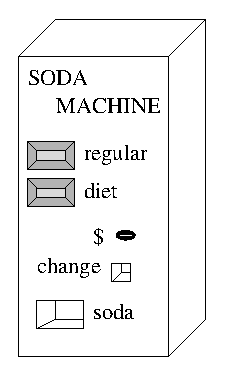
\includegraphics{Prob7-4}}
            \caption{A basic vending machine.}
            \label{fig:Vend}
        \end{figure}\vspace{-1em}
        \begin{onlysolution}  \textbf{Solution} \itshape{
                \begin{figure}[ht]
                    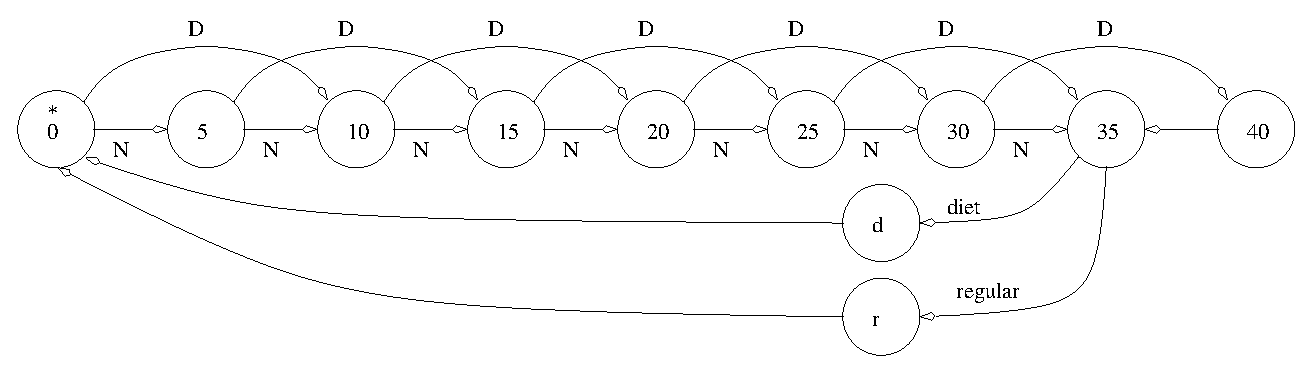
\includegraphics[max width=\textwidth, center]{Sol7-4}
                \end{figure}

                Note, that in the figure if a input does not appear on
                any arc emanating from a state then it is implied that
                this input will have no effect on the next state.  Below
                are the outputs for each of the states above.

                \begin{tabular}{|l||l|l|l|} \hline
                    \multicolumn{4}{|c|}{outputs from the vending FSM}                      \\ \hline \hline
                    state   & nickel change     & diet dispense     & regular dispense      \\ \hline
                    & 0 give none       & 0 give none       & 0 given none          \\ \hline
                    & 1 give nickel     & 1 dispense diet   & 1 dispense regular    \\ \hline
                    &                   &                   &                       \\ \hline
                    0       & 0                 & 0                 & 0                     \\ \hline
                    5       & 0                 & 0                 & 0                     \\ \hline
                    10      & 0                 & 0                 & 0                     \\ \hline
                    15      & 0                 & 0                 & 0                     \\ \hline
                    20      & 0                 & 0                 & 0                     \\ \hline
                    25      & 0                 & 0                 & 0                     \\ \hline
                    30      & 0                 & 0                 & 0                     \\ \hline
                    35      & 0                 & 0                 & 0                     \\ \hline
                    40      & 1                 & 0                 & 0                     \\ \hline
                    d       & 0                 & 1                 & 0                     \\ \hline
                    r       & 0                 & 0                 & 1                     \\ \hline
                \end{tabular}
            }
        \end{onlysolution}

    \item \textbf{ (6 pts.)}
        Build a FSM for a car alarm.  The input to the FSM
        comes from a tilt sensor.  The tilt-sensor outputs 1 when the
        car has been physically displaced by a preset amount, otherwise the
        tilt sensor outputs 0.  The output of the circuit drives an alarm,
        when the alarm output equals 1 the alarm sounds, otherwise the alarm
        does not sound.  Once the alarm has been set off, it will continue
        sounding until a reset input equals 1, at which point the alarm will
        stop sounding.

        Draw the state diagram and from this determine the MIEs and OEs.

        \begin{onlysolution}
            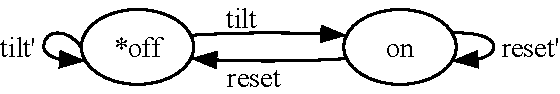
\includegraphics[center]{Sol7-5}
            \textbf{MIE:}
            \begin{flalign*}
                D_{off} &= Q_{off}Tilt' +  Q_{on}Reset &&\\
                D_{on}  &= Q_{off}Tilt\  + Q_{on}Reset' &&
            \end{flalign*}
            \textbf{OE:}
            \begin{flalign*}
                Alarm\ &= D_{on}  &&\\
                Alarm' &= D_{off} &&
            \end{flalign*}
        \end{onlysolution}
    \item \textbf{ (12 pts.)}
        Build a digital circuit which controls an automatic garage door opener.
        The garage door circuit has three bits of input.  The first input, called
        $button$, comes from a the main control button used to open or close the
        garage door.  When pressed $button=1$ otherwise $button=0$.  The garage
        door rides in a track, at the top and bottom of of which are two
        limit switches.  The top limit switch equals 1 when the garage door
        is all the way up, otherwise its output equals 0.  The bottom limit
        switch equals 1 when the garage door is all the way down, otherwise
        its output equals 0.  The garage door circuit has two bits of output
        called $motor$.  When $motor=01$, the motor moves the door in a downward
        motion, closing the door.  When $motor=10$, the motor moves the door
        upward, opening the garage door.  When $motor=00$, the motor is turned off.

        \begin{figure}[ht]
            \center{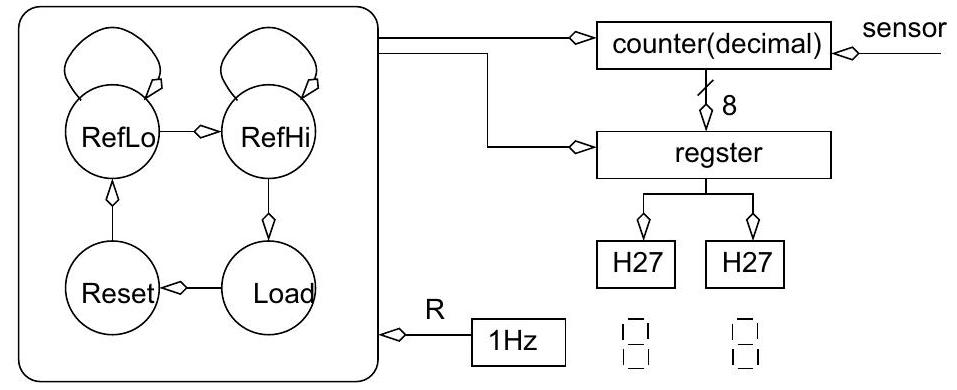
\includegraphics{Prob7-6}}
            \caption{The garage door and the circuit controlling it.}
            \label{fig:hwgarage}
        \end{figure}

        Construct the FSM assuming a one-hot encoding of the states.
        Determine the memory input equations and output equations.

        \begin{onlysolution}  \textbf{Solution:} \itshape{
                \begin{itemize}
                    \item\textbf{Control unit}
                        The control unit includes so called wait states.  Waits states are
                        a result of the fact that the clock running the FSM is usually
                        much faster than the physical phenomena being monitored by the FSM.
                        Unless told otherwise, you can assume that any FSM that you are
                        building has a clock which operates on the order of megahertzs.
                        This means that the resulting FSM can make around 1 million
                        state transitions per second.  Clearly, a garage door needs more
                        than one millionth of a second to open or close.  Consequently,
                        the FSM in this problem needs to wait for the door to be opened.
                        This is done by having the FSM repetitively check the status of the
                        door via the up or down limit switches.  In addition to waiting
                        for the garage door to open and close the FSM must wait for a
                        button press.

                        \begin{figure}[ht]
                            \center{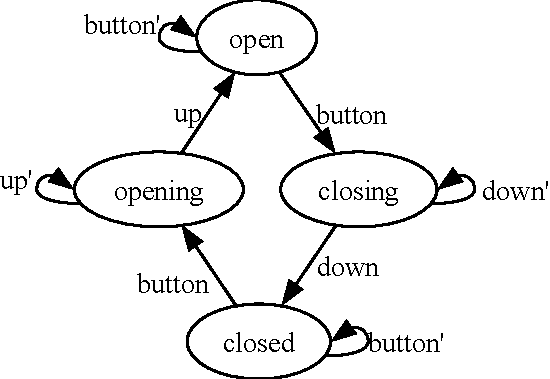
\includegraphics{Sol7-6}}
                            \caption{The FSM for the garage door controller.}
                        \end{figure}

                        The state diagram for the garage door controller has four states.
                        In the open and close state, the FSM is waiting for a button push,
                        while the button is not pressed the door stays open or closed.  As
                        soon as the button is pressed the door starts to open or close.
                        It stays in this state until the limit switches tell the FSM that
                        the door has reached the limit of its travel.

                    \item\textbf{Memory Input Equations}
                        Since we are building the garage door controller assuming a
                        one hot encoding of the states, each state will get its own
                        flip flop.  Each flip flop will output a 1 when the FSM is
                        in that state.  The memory input equations for a particular
                        state are determined by answering, ``how do you get into that
                        state?" The four answers to this questions are provided below.

                        {\addtolength{\tabcolsep}{-0.4em}
                            \begin{tabular}{lll}
                                $D_{open}     $&$=\, Q_{open}button'  $&$+\, Q_{opening}up$ \\
                                $D_{close}    $&$=\, Q_{close}button' $&$+\, Q_{closing}down$ \\
                                $D_{opening}  $&$=\, Q_{close}button  $&$+\, Q_{opening}up'$ \\
                                $D_{closing}  $&$=\, Q_{open}button   $&$+\, Q_{closing}down'$ \\
                        \end{tabular}}

                    \item\textbf{Output Equations}
                        The outputs for complex FSMs are usually not written inside the
                        states, rather a separate table is constructed which contains the
                        output for each state.   Even though this is a simple example
                        we will construct an output table.

                        \begin{tabular}{l|l}
                            State    & motor        \\ \hline
                            & 00 stop    \\ \hline
                            & 01 down    \\ \hline
                            & 10 up        \\ \hline
                            open    & 00         \\ \hline
                            close   & 00        \\ \hline
                            opening & 10         \\ \hline
                            closing & 01         \\
                        \end{tabular}

                        Call the outputs $Z_{m1}$ and $Z_{m0}$, for the most and least
                        significant bits of the output respectively.  Then the outputs
                        are determined by asking for which states does the output
                        equal 1?  The answers to this question are shown below.

                        \begin{tabular}{l}
                            $Z_{m1} = Q_{opening}$ \\
                            $Z_{m0} = Q_{closing}$ \\
                        \end{tabular}
                \end{itemize}
            }
        \end{onlysolution}

    \item \textbf{ (8 pts.)}
        Build a digital circuit to control a single traffic light.  The circuit
        has three outputs, $Rlight, Ylight$ and $ Glight$.  When
        $Rlight=1$ the red light illuminates otherwise the light is off.
        The same behavior holds true for $Ylight$ and $Glight$.  In order
        to sequence the lights, the circuit has three timers, Rtimer, Gtimer and
        Ytimer.  Each timer controls the length of time that its light should be
        illuminated.  Each timer has one bit of input and one bit of output.  When a
        timer's input is 0, the timer is reset.  When a timer's one bit
        input is 1, the timer
        counts down its preset timer interval.  When a timer counts all the way down,
        its output goes to 1 and stays there until the timer is reset (by applying
        an input of 0).  The state diagram of the circuit is shown in the
        figure below.  As shown in figure~\ref{fig:TrafficFSM} the FSM receives input from the
        three timers, while the output of the FSM controls the counters. Complete
        the following three tasks.
        \begin{figure}[t]
            \ifshowanswers 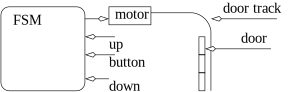
\includegraphics[max width=\textwidth, center]{Sol7-7}
            \else 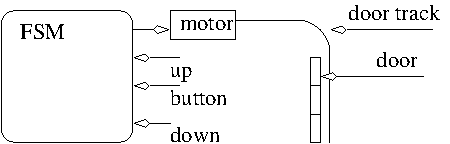
\includegraphics[max width=\textwidth, center]{Prob7-7} \fi
            \caption{}
            \label{fig:TrafficFSM}
        \end{figure}

        \begin{enumerate}
            \item Label the arcs of the FSM with the input values (Rt, Yt or Gt)
                needed to make the circuit operate correctly.

            \item Next, determine what the output should be in each
                of the states.  Instead of writing the output in each state, the
                outputs are organized in a separate table.  In this table, each
                row will contain the output associated with a particular state.
                Each column in the table will be associated with one bit of the output.

                \begin{onlyproblem}
                    \begin{tabular}{l||l|l|l|l|l|l}state&Rlight&Ylight&Glight&Rtimer&Ytimer&Gtimer\\\hline&0~off&0~off&0~off&0~rst&0~rst&0~rst\\\hline&1~on&1~on&1~on&1~run&1~run&1~run\\\hline\hline R&&&&&&\\\hline Y&&&&&&\\\hline G&&&&&&\\
                    \end{tabular}
                \end{onlyproblem}
                \begin{onlysolution}
                    \begin{tabular}{l||l|l|l|l|l|l}
                        state         & Rlight & Ylight & Glight & Rtimer & Ytimer & Gtimer    \\ \hline
                        & 0 off  & 0 off  & 0 off  & 0 rst  & 0 rst  & 0 rst    \\ \hline
                        & 1 on   & 1 on   & 1 on   & 1 run  & 1 run  & 1 run    \\ \hline \hline
                        R             & 1      & 0      & 0      & 1      & 0      & 0        \\ \hline
                        Y             & 0      & 1      & 0      & 0      & 1      & 0        \\ \hline
                        G             & 0      & 0      & 1      & 0      & 0      & 1        \\
                    \end{tabular}
                \end{onlysolution}

            \item Finally, write the memory input equations and output
                equations for the traffic light controller.  In order to write the
                memory input equations use the labels on the state transitions from
                the state diagram.   In order to write the output equations
                use the output table.

                \begin{onlyproblem}
                    \begin{tabular}{p{2in}p{2in}}
                        \begin{tabular}{l@{}l}$Q_{red}$&$=$\\$Q_{yellow}\,$&$=$\\$Q_{green}$&$=$\\
                        \end{tabular}&
                        \begin{tabular}{l@{}l}$Z_{Rlight}$&$=$\\$Z_{Ylight}$&$=$\\$Z_{Glight}$&$=$\\$Z_{Rtimer}$&$=$\\$Z_{Ytimer}$&$=$\\$Z_{Gtimer}\,$&$=$\\
                        \end{tabular}
                    \end{tabular}
                \end{onlyproblem}
                \begin{onlysolution}{\color{blue}
                        \begin{tabular}{p{2in}p{2in}}
                            \begin{tabular}{l@{}l} % @{} removes all automatic padding from the table
                                $D_{red}$      & $=Q_{Set30} + Q_{Red   }Rt$    \\
                                $D_{yellow}\,$ & $=Q_{Set5 } + Q_{Yellow}Yt$    \\ % Manually creating alignment removes the spacing around symbols, so artificially add it back on longest line
                                $D_{green}$    & $=Q_{Set25} + Q_{Green }Gt$    \\
                            \end{tabular}
                            &
                            \begin{tabular}{l@{}l}
                                $Z_{Rlight}$   & $= Q_{Red   }$ \\
                                $Z_{Ylight}$   & $= Q_{Yellow}$ \\
                                $Z_{Glight}$   & $= Q_{Green }$ \\
                                $Z_{Rtimer}$   & $= Q_{Red   }$ \\
                                $Z_{Ytimer}$   & $= Q_{Yellow}$ \\
                                $Z_{Gtimer}\,$ & $= Q_{Green }$ \\
                            \end{tabular}
                    \end{tabular}}
                \end{onlysolution}
        \end{enumerate}
        \filbreak
    \item \textbf{ (16 pts.)}
        Build a FSM which make the hexapod robot shown in Figure~\ref{fig:hexapod}
        walk forward.

        \begin{figure}[ht]
            \center{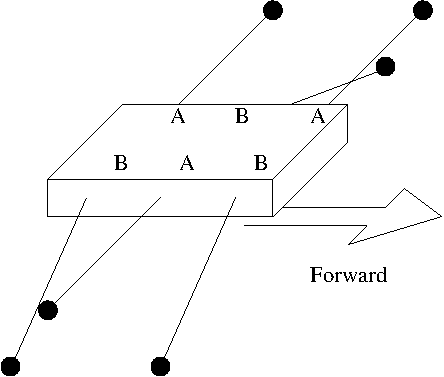
\includegraphics{Prob7-8}}
            \caption{A hexapod walking robot.}
            \label{fig:hexapod}
        \end{figure}

        Each leg of the hexapod robot is moved by two nitinol (Flexinol) wires.
        At rest, nitinol wire is straight.  When 5 volts (logic 1) is applied to
        the wire, it bends in a particular direction.  The two wires making up
        a particular leg are positioned so that they move in perpendicular
        directions.  One wire moves a leg up or down and the other will move
        the wire forward or backwards.  The table below elaborates.

        \begin{tabular}{l|l|l}
            wire   & logic 0 & logic 1    \\ \hline
            $w_0$  & down     & up        \\ \hline
            $w_1$  & forward & backward    \\
        \end{tabular}

        The hexapod robot walks by moving three legs in unison; see $A$ and
        $B$ in Figure~\ref{fig:hexapod}.  The movements of $A$ and $B$ are
        coordinated so that, at times, the hexapod is balanced on three legs.
        A portion of the walking gait is shown in Figure~\ref{fig:hexgate};
        note that in this figure the viewer is looking down at the top of the
        robot which is moving to the right.  The dotted legs are assumed to be in
        the air, solid legs are in contact with the ground.

        \begin{figure}[ht]
            \center{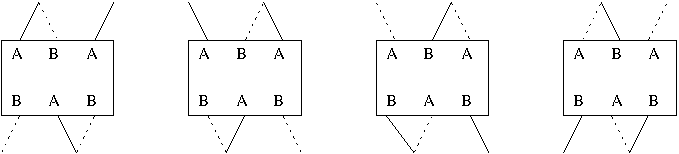
\includegraphics{Prob7-8b}}
            \caption{The walking gait of the hexapod robot.}
            \label{fig:hexgate}
        \end{figure}

        Assume that the legs can move to their correct position in one clock
        cycle.  Define each state as a position of the legs in
        Figure~\ref{fig:hexgate}. Draw the state diagram,
        and determine the memory input and output equations.

        \begin{onlysolution}\filbreak  \textbf{Solution} \itshape{

                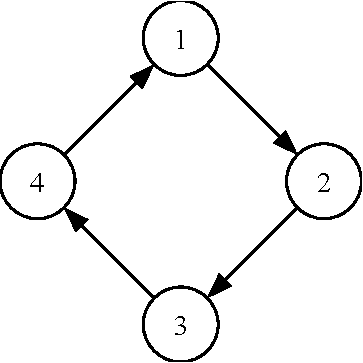
\includegraphics[max width=\textwidth, center]{Sol7-8}
                Note that the states have been given numbers to simplify the
                description of the states.  Here is a listing of the outputs
                associated with each state:

                \begin{tabular}{l|l|l|l|l}
                    State  & $Aw_1$ & $Aw_0$ & $Bw_1$ & $Bw_0$  \\ \hline
                    1    & 0    & 0     & 1      & 1        \\ \hline
                    2    & 1    & 0     & 0      & 1        \\ \hline
                    3    & 1    & 1     & 0      & 0        \\ \hline
                    4    & 0    & 1     & 1      & 0        \\
                \end{tabular}

                \textbf{ MIEs and OEs}

                \begin{tabular}{ll}
                    MIEs        &    OEs            \\
                    $D_1 = Q_4$    &    $Z_{Aw_1} = Q_2 + Q_3$    \\
                    $D_2 = Q_1$    &    $Z_{Aw_0} = Q_3 + Q_4$    \\
                    $D_3 = Q_2$    &    $Z_{Bw_1} = Q_1 + Q_4$    \\
                    $D_4 = Q_3$    &    $Z_{Bw_0} = Q_1 + Q_2$    \\
                \end{tabular}

            }
        \end{onlysolution}

    \item \textbf{ (12 pts.)}
        \label{item:robot}
        Build a FSM which makes the simple robot shown in Figure~\ref{fig:Robot}
        move along (track) the black line crossing two intersections.
        \begin{figure}[ht]
            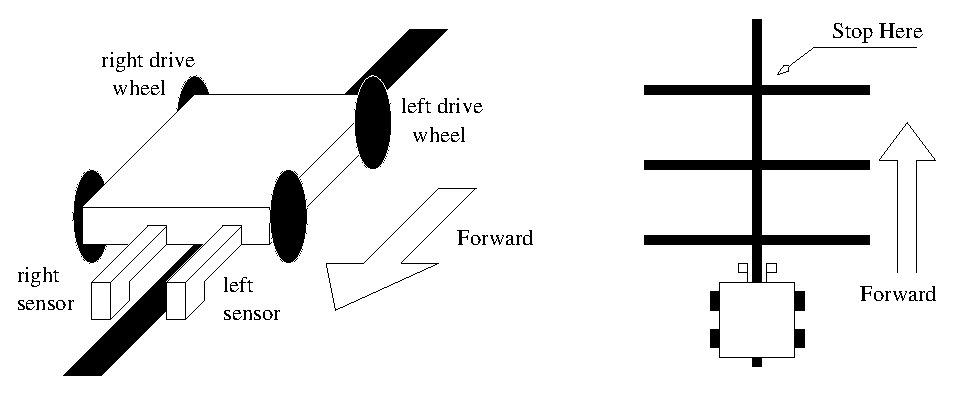
\includegraphics[max width=\textwidth, center]{Prob7-9}
            \caption{A simple line-tracking robot that must cross two intersections.}
            \label{fig:Robot}
        \end{figure}

        The FSM has two inputs, a left sensor, denoted \textit{ ls}, and a right
        sensor, denoted \textit{ rs}.  These two sensors look down at the ground.
        When a sensor sees white, it outputs 0; when it see black, it outputs 1.
        The sensors are spaced far enough apart that they can straddle the black
        line and see white on either side.  The FSM has two outputs, a left
        motor, denoted \textit{ lm} and a right motor, denoted \textit{ rm}.  A motor
        rotates when it is sent a 1 and does not rotate when it is sent a 0.
        The FSM should constantly check that the robot is straddling the line.
        If it is not the FSM should take corrective action by stopping one of
        the wheels.

        Submit the state diagram for the FSM,  MIEs and OEs using
        a one-hot encoding of the states.

        \begin{onlysolution}  \textbf{Solution} \itshape{

                \textbf{FSM}

                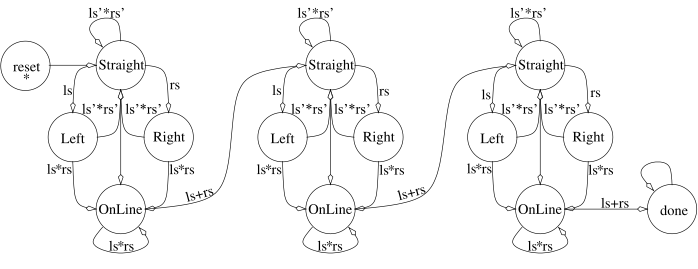
\includegraphics[max width=\textwidth, center]{Sol7-9}
                \begin{tabular}{l|l|l|l}
                    State    & lm                & rm                  \\ \hline
                    & 0 stop left wheel & 0 stop right wheel  \\ \hline
                    & 1 turn left wheel & 1 turn right wheel  \\ \hline
                    &                   &                     \\ \hline \hline
                    Reset    & 1                 & 1                   \\ \hline
                    Straight & 1                 & 1                   \\ \hline
                    Left     & 0                 & 1                   \\ \hline
                    Right    & 1                 & 0                   \\ \hline
                    OnLine   & 1                 & 1                   \\ \hline
                    Done     & 0                 & 0                   \\
                \end{tabular}
            }
            {\color{blue}
                \textbf{MIE}
                \begin{align*}
                    D_{S }    &= Q_{Reset} + Q_{S}(ls'*rs') + Q_{L}(ls'*rs') + Q_{R}(ls'*rs') + Q_{OL}(ls+rs)\\
                    D_{L }    &= Q_{S}(ls*rs') \\
                    D_{R }    &= Q_{S}(ls'*rs) \\
                    D_{OL}    &= Q_{L}(ls*rs)  + Q_{R}(ls*rs) + Q_{S}(ls*rs) + Q_{OL}(ls*rs)\\
                    D_{Done} &=  Q_{OL}(ls+rs) + Q_{Done}
                \end{align*}
                \textbf{OE}
                \begin{align*}
                    Z_{lm} &= Q_{Reset} + Q_{S} + Q_{R} + Q_{OL}\\
                    Z_{rm} &= Q_{Reset} + Q_{S} + Q_{L} + Q_{OL}
            \end{align*}}
        \end{onlysolution}

    \item \textbf{ (16 pts.)}
        Make the robot from Problem \ref{item:robot} cross 63 intersections.
        The problem is that the number of states will grow to large to handle
        with a FSM by itself.  Additional hardware, in the form of a counter
        and comparator, are added to the FSM to address this problem.

        \begin{figure}[ht]
            \center{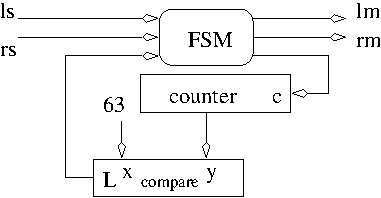
\includegraphics[max width=\textwidth, center]{Prob7-10}}
            \caption{The innards of a intersection counting, line tracking robot.}
            \label{fig:linecounter}
        \end{figure}

        Assume that the counter is reset to 0 when the circuit
        is first turned on.  The robot must still track the line, but
        must also count up once every time it crosses an intersection.  Remember
        the digital circuit shown in Figure~\ref{fig:linecounter} is
        operating much faster than the robot is crossing intersections.
        \filbreak
        The state diagram needs to have wait states while it crosses
        the intersection, similar to those
        in the DAISY example.  Assume the counter counts up
        when the control input is 1 and the clock rises.  When the control
        input is 0, then the counter holds its current count value.

        Submit the state diagram for the FSM, OEs and MIEs for a one-hot
        encoding of the states.

        \begin{onlysolution}  \textbf{Solution} \itshape{
                If you encoded 64 line crossing using only a FSM you would have
                on the order of 256 states, 4 for each line crossing.  The solution
                is to use a counter to keep track of how many lines have been crossed.
                The states below explain.

                \textbf{FSM}

                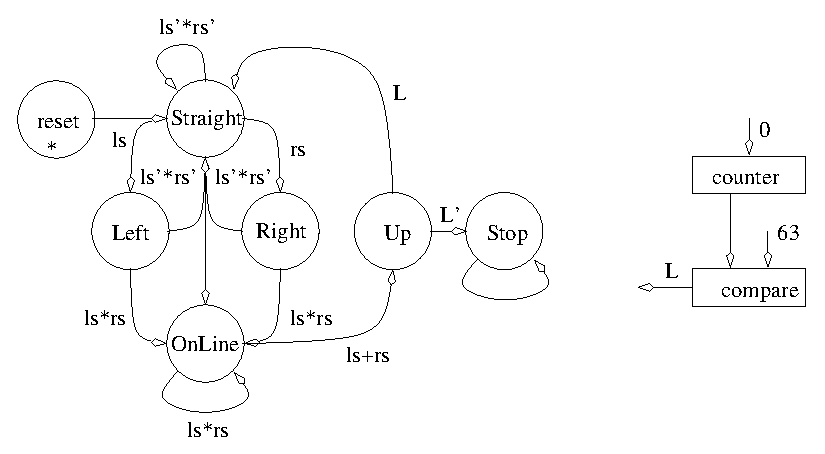
\includegraphics[max width=\textwidth, center]{Sol7-10}

                \filbreak
                \textbf{ Control Word}

                \begin{tabular}{l|l|l|l}
                    State    & lm                & rm                  & counter \\ \hline
                    & 0 stop left wheel & 0 stop right wheel  & 00 hold \\ \hline
                    & 1 turn left wheel & 1 turn right wheel  & 01 load \\ \hline
                    &                   &                     & 10 count\\ \hline \hline
                    Reset    & 1                 & 1                   & 01      \\ \hline
                    Straight & 1                 & 1                   & 00      \\ \hline
                    Left     & 0                 & 1                   & 00      \\ \hline
                    Right    & 1                 & 0                   & 00      \\ \hline
                    OnLine   & 1                 & 1                   & 00      \\ \hline
                    Up       & 1                 & 1                   & 10      \\ \hline
                    Stop     & 0                 & 0                   & 00      \\
                \end{tabular}

                { \color{blue}
                    \textbf{MIE}
                    \begin{flalign*} % flalign both sets as these are almost the width of the page
                        D_{S }   &= Q_{Reset} + Q_{S}(ls'*rs') + Q_{L}(ls'*rs') + Q_{R}(ls'*rs') + Q_{Up}(L)\\
                        D_{L }   &= Q_{S} (ls*rs') \\
                        D_{R }   &= Q_{S} (ls'*rs) \\
                        D_{OL}   &= Q_{L} (ls*rs)  + Q_{R}(ls*rs) + Q_{S}(ls*rs) + Q_{OL}(ls*rs)\\
                        D_{Up}   &= Q_{OL}(ls+rs)  &\\
                        D_{Stop} &= Q_{Up}(L') &
                    \end{flalign*}
                    \textbf{OE}
                    \begin{flalign*}
                        Z_{lm } &= Q_{Reset} + Q_{S} + Q_{R}  + Q_{OL} &\\
                        Z_{rm } &= Q_{Reset} + Q_{S} + Q_{L}  + Q_{OL} &\\
                        Z_{c_1} &= Q_{Up} & \\
                        Z_{c_0} &= Q_{Reset} &
                \end{flalign*}}
            }
        \end{onlysolution}

    \item \textbf{ (24 pts.)}
        Construct a digital circuit to control the operation of a
        simple washing machine, see Figure~\ref{fig:Wash}.
        \begin{figure}[ht]
            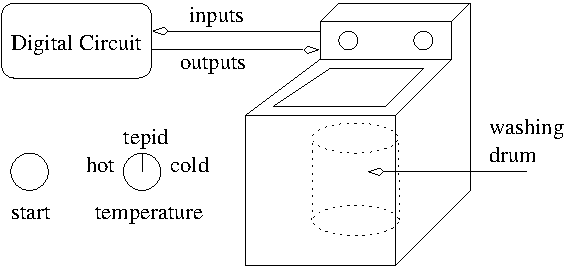
\includegraphics[max width=\textwidth, center]{Prob7-11}
            \caption{A humble washing machine with a close-up of the start
            button and temperature switch.}
            \label{fig:Wash}
        \end{figure}

        To use the simple washing machine set the temperature switch to
        either hot, tepid or cold and then press the start button.
        To build a digital circuit to control the washing of clothes
        its necessary to understand the washing cycle.  When the start
        button is pressed water of the selected temperature pours
        into the washing drum.  The simple washing machine has two
        electronically controlled water valves, the hot valve admits
        hot water into the washing drum and the cold valve admits
        cold water.  Water continues to pour into the drum until it
        fills.  There are two water level sensors; the full switch signals when
        the drum is full of water and the empty switch signals when the drum
        is empty.  After the drum is full of water the simple washing machine
        starts to agitate the clothes.  The simple washing machine has a motor
        controlled by two bits, which agitates (a rapid back and forth motion),
        spins (a rapid rotation in one direction) or does nothing.  After
        agitating for 15 minutes, the agitation cycle stops and
        the machine drains its water.  Water leaves the drum through
        a drain valve.  When the drum is emptied of water the washing machine enters
        the rinse cycle.   The rinse cycle fills the drum with cold
        water and agitates for 5 minutes.  The rinse cycle concludes
        by draining the water from the drum.
        When the drum is emptied of water the washing machine enters
        the spin cycle.  This lasts for 5 minutes.  The simple washing machine
        keeps track of time  using a 5 minute timer.   To use the timer
        it must first be reset for one clock cycle.  After being reset the
        timer will count down as long as the timer input is set to run.
        After 5 minutes have elapsed the timer output will go to logic 1 and
        stay there until the timer is reset.  In order to get longer time
        intervals, the timer should be reset for another 5 minutes and count
        down again.  When the spin cycle is done, the washing is complete. The
        inputs from the washing machine to the digital circuit have the
        following meaning.

        \begin{tabular}{|l|l|l|l|l|} \hline
            \multicolumn{5}{|c|}{inputs to the digital circuit}        \\ \hline \hline
            start & temperature & empty       & full       & timer out     \\ \hline
            0 off & 00 hot      & 0 not empty & 0 not full & 0 nothing    \\ \hline
            1 on  & 01 cold     & 1 empty     & 1 full     & 1 5 minutes elapsed     \\ \hline
            & 10 tepid    &          &           &        \\ \hline
        \end{tabular}

        The outputs from the digital to the washing machine have the following meaning.
        The left most column is explained below.

        \begin{tabular}{|l|||l|l|l|l|l|} \hline
            \multicolumn{6}{|c|}{outputs from the digital circuit}            \\ \hline \hline
            state & hot     & cold    & motor      & timer in   & drain     \\ \hline
            & 0 close & 0 close & 00 off     & 00 hold    & 0 close    \\ \hline
            & 1 open  & 1 open  & 01 agitate & 01 reset   & 1 open    \\ \hline
            &        &         & 10 spin    & 10 run     &        \\ \hline \hline
            \textbf{ S1}    &    &      &           &        &        \\ \hline
        \end{tabular}

        Draw the state diagram for the FSM to control the washing machine.
        Label the arcs of the state diagram with the input (or its negation)
        that causes the transition.  Use simple Boolean expressions on these
        arcs, for example (start and hot).
        For each state define the output using a table similar to the one above.
        For example, if \textbf{ S1} is a state fill in the bit values for the o
        outputs depending on what state \textbf{ S1} is supposed to do.
        Determine the memory input equations and output equations assuming a one-hot
        encoding.

        \begin{onlysolution}  \textbf{Solution} \itshape{
                % \begin{enumerate} % I'm not sure what most of these mean, or why these are the only deductions listed for any problem
                %     \item No control table (-6)
                %     \item Disposable washing machine (-1)
                %     \item No OEs (-5)
                %     \item start * cold (-2)
                %     \item no complements on arcs (-2)
                % \end{enumerate}
                \begin{figure}[ht]
                    \center{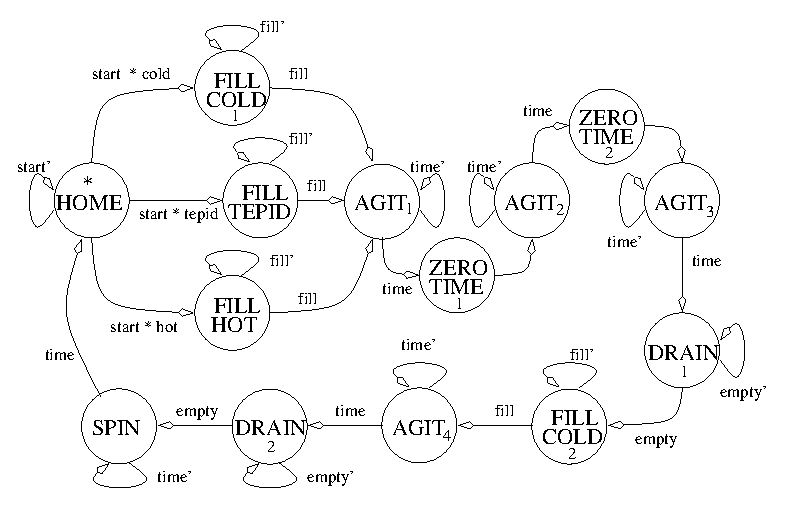
\includegraphics{Sol7-11}}
                    \caption{The FSM for a washing machine.}
                \end{figure}

                \begin{tabular}{|l|||l|l|l|l|l|} \hline
                    \multicolumn{6}{|c|}{outputs from the digital circuit}        \\ \hline \hline
                    state & hot     & cold    & motor      & timer in   & drain   \\ \hline
                    & 0 close & 0 close & 00 off     & 00 nothing & 0 close \\ \hline
                    & 1 open  & 1 open  & 01 agitate & 01 reset   & 1 open  \\ \hline
                    &         &         & 10 spin    & 10 start   &         \\ \hline
                    &         &         &            & 11 stop    &         \\ \hline \hline
                    HOME  &    0    & 0       & 00         & 00         & 0       \\ \hline
                    COLD  &    0    & 1       & 00         & 01         & 0       \\ \hline
                    TEPI  &    1    & 1       & 00         & 01         & 0       \\ \hline
                    HOT   &    1    & 0       & 00         & 01         & 0       \\ \hline
                    AGIT  &    0    & 0       & 01         & 10         & 0       \\ \hline
                    ZERO  &    0    & 0       & 00         & 01         & 0       \\ \hline
                    DRAI  &    0    & 0       & 00         & 01         & 1       \\ \hline
                    SPIN  &    0    & 0       & 10         & 10         & 0       \\ \hline
                \end{tabular}
                \begin{align*}
                    D_{home}   &= Q_{home}start' + Q_{spin}time \\
                    D_{cold1}  &= Q_{home}*start*cold \\
                    D_{tepi}   &= Q_{home}*start*tepid \\
                    D_{hot}    &= Q_{home}*start*hot \\
                    D_{agit1}  &= Q_{cold1}*fill + Q_{tepid}*fill + Q_{hit}*fill + Q_{agit1}*time' \\
                    D_{zero1}  &= Q_{agit1}*time \\
                    D_{agit2}  &= Q_{zero1}*time + Q_{agit2}*time' \\
                    D_{zero2}  &= Q_{agit2}*time \\
                    D_{agit3}  &= Q_{zero2}*time + Q_{agit2}*time' \\
                    D_{drain1} &= Q_{agit3}*time + Q_{drain1}*empty' \\
                    D_{cold2}  &= Q_{drain1}*empty + Q_{cold2}*fill' \\
                    D_{agit4}  &= Q_{cold2}*fill + Q_{agit4}*time' \\
                    D_{drain2} &= Q_{agit4}*time + Q_{drain2}*empty' \\
                    D_{spin}   &= Q_{drain2}*empty + Q_{spin}*time'
                \end{align*}

                {\color{blue}
                    \begin{align*}
                        Z_{hot    } &= Q_{tepid} + Q_{hot}\\
                        Z_{cold   } &= Q_{cold} + Q_{tepid}\\
                        Z_{motor_1} &= Q_{spin}\\
                        Z_{motor_0} &= Q_{agit}\\
                        Z_{timer_1} &= Q_{agit} + Q_{spin}\\
                        Z_{timer_0} &= Q_{cold} + Q_{tepid} + Q_{hot} + Q_{zero} + Q_{drain}\\
                        Z_{drain  } &= Q_{drain}
                \end{align*}}
            }
        \end{onlysolution}

    \item \textbf{ (36 pts.)}
        Construct a digital circuit to control the movement of an elevator in a
        four-story building.  The elevator will always wait on its current floor
        until a call button is pressed; see Figure~\ref{fig:elevator}.  The
        elevator then moves to the floor that was called.  The elevator then
        opens its doors and waits for an elevator control button to be pressed.
        If a a call to another floor is received before an elevator control
        button is pressed, then the elevator closes the doors and goes to the
        new floor.  When a floor is selected on the elevator control panel, then
        the door close and the elevator moves to the desired floor.

        \begin{figure}[ht]
            \center{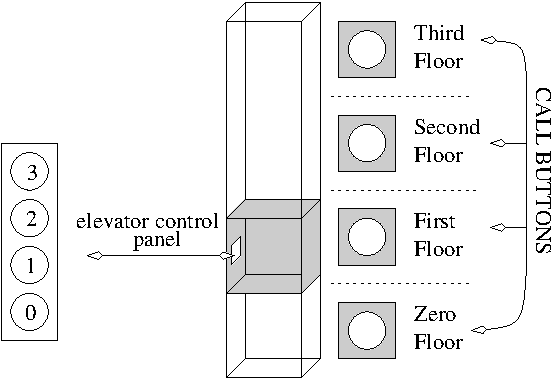
\includegraphics{Prob7-12}}
            \caption{The layout of an elevator in a four story tall building.}
            \label{fig:elevator}
        \end{figure}

        The inputs to the digital circuit clearly include all the buttons.
        When a button is pressed on the elevators control panel two things
        happen.  A 2-bit binary value representing the button pressed
        becomes valid and a 1-bit panel request becomes valid.  The
        panel request line will remain valid until acknowledged.

        When a call button is pressed two things happen.  A 2-bit binary value
        representing which call button was pressed becomes valid and a 1-bit
        call request becomes valid.  The call request line will remain valid
        until acknowledged.

        Another input tells the circuit when the
        elevator is or is not aligned with a floor.  For example, consider
        an elevator moving from the first to the third floor.  Initially, the
        align variable is 1.  When the elevator starts
        to move away from the first floor towards the second, the align
        variable goes to 0.  When the elevator reaches the second floor, the
        align variable will go to logic 1 and remain there for a short
        while (at least several milliseconds) because there is some
        slack allowed in what is considered ``aligned".  After the elevator
        passes the second floor, the align variable goes back to 0 and stays
        there until the elevator reaches the third floor.

        Here is the table of inputs to the FSM, their abbreviations, to be
        used in the FSM, and their meaning.

        \begin{tabular}{|l|l||l|l|} \hline
            Control panel floor     & Pfloor        & 2-bit floor number & \\ \hline
            Panel request           & Preq          & The panel has a valid floor & \\ \hline
            Call floor              & Cfloor        & 2-bit floor number & \\ \hline
            Call request            & Creq          & The call buttons have a valid floor & \\ \hline
            Align                   & Align         & 0 not aligned & 1 Aligned \\ \hline
        \end{tabular}

        The outputs from the digital circuit to control the door and the
        movement of the elevator.

        \begin{tabular}{|l|l|l|l|} \hline
            Panel acknowledge       & Pack  & Acknowledge the panel request & \\ \hline
            Call acknowledge        & Cack  & Acknowledge the call request & \\ \hline
            Door                    &  0 close &    1 open  &         \\ \hline
            Motor                   &  00 stop &    01 up   & 10 down \\ \hline
        \end{tabular}

        Submit; an algorithm for the datapath and control unit,
        the control word table, the memory input equations, and output equations.
        \begin{onlysolution}[fragile] \color{blue}\par%fragile required to use verbatim environments inside of an answer
            \textbf{Algorithm}
\begin{lstlisting}
int loc;
int delta;
while(1) {
    if(Creq){
        Cack = 1;
        Door = 0;
        delta = Cfloor - loc;
        loc = Cfloor;
        Cack = 0;
    }
    if(Preq){
        Pack = 1;
        Door = 0;
        delta = Pfloor - loc;
        loc = Pfloor;
        Pack = 0;
    }
    if delta != 0 {
        if (delta > 0) { // elevator needs to go up
            while (delta > 0){
                while(align == 1){Motor = 01;} // Keep powered
                delta = delta - 1;
                while(align == 0){Motor = 01;} // Wait until aligned
            }
        }
        else if (delta < 0) { // elevator needs to go down
            while (delta < 0){
                while(align == 1){Motor = 10;}
                delta = delta + 1;
                while(align == 0){Motor = 10;}
            }
        }
        Motor = 00;
        Door = 1;
    }
}
\end{lstlisting}
            \textbf{Datapath and Control}

            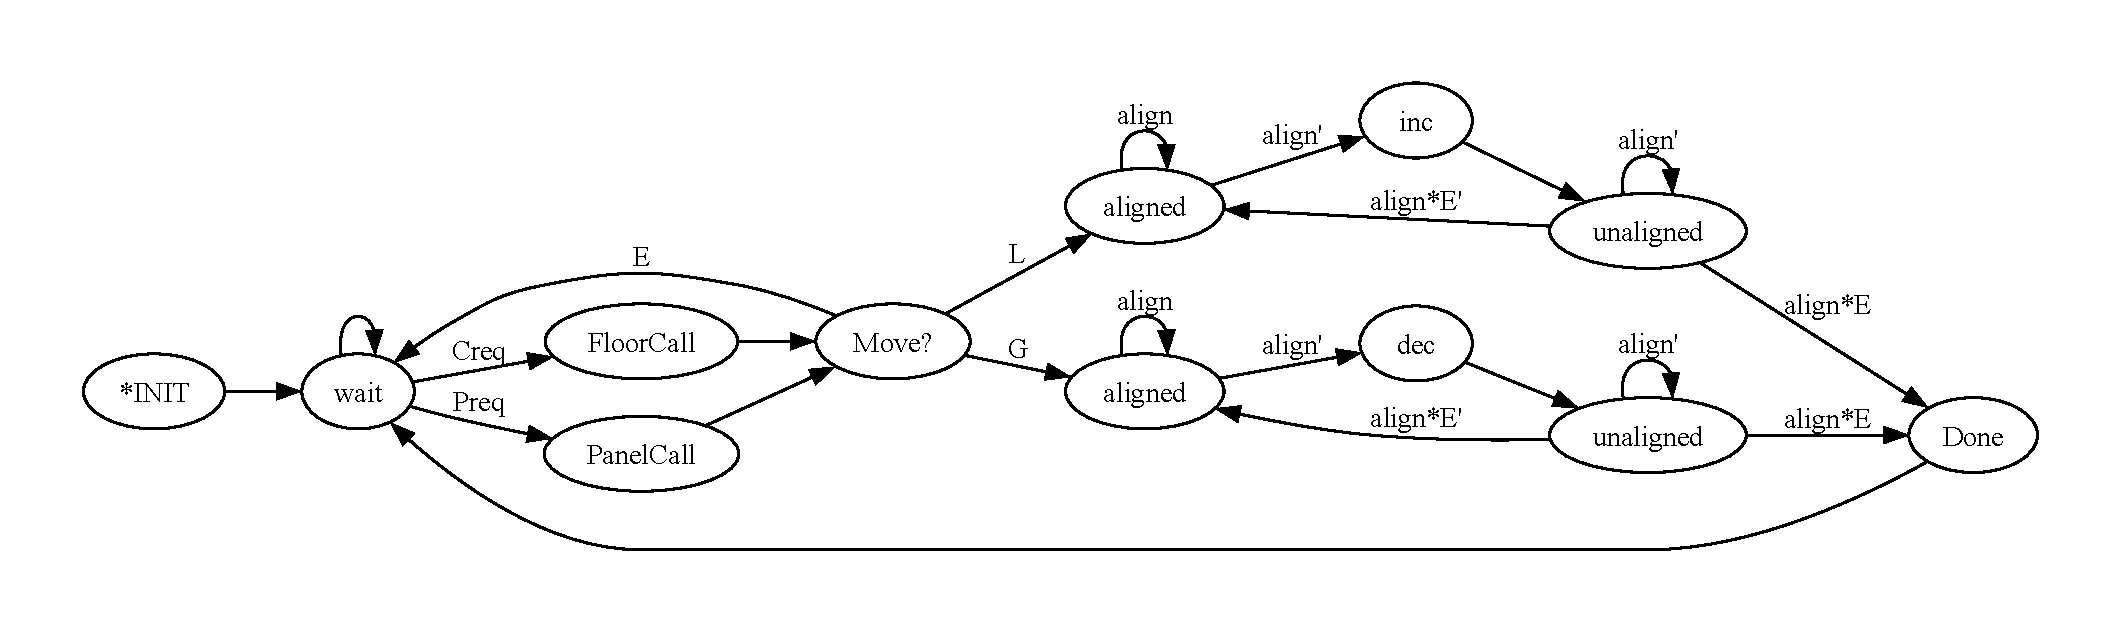
\includegraphics[max width=\textwidth, center]{sol7-12}
            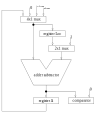
\includegraphics[max width=\textwidth, center]{sol7-12DP}
            \textbf{Control Words}
            \begin{tabular}{c}
            \end{tabular}
        \end{onlysolution}
    \item \textbf{ (36 pts.)}
        Construct a digital circuit to control the movement of traffic
        at the four way intersection shown in Figure~\ref{fig:crossroad}.

        \begin{figure}[ht]
            \center{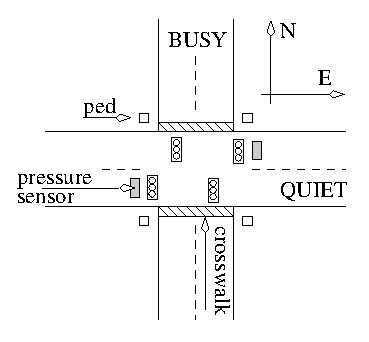
\includegraphics{Prob7-13}}
            \caption{The layout of a four way intersection.}
            \label{fig:crossroad}
        \end{figure}

        The circuit comes equipped with timers.
        The timer has 2 inputs which set the timer to some preset
        amount of time or allows the timer to count down.  When the
        timer reaches 0 then the output of the timer goes to 1.
        When the timer is not at 0 then the output equals 1.
        The specific inputs and behavior are described in the following
        truth table.

        \begin{tabular}{|c|c|} \hline
            timer input & behavior          \\ \hline \hline
            00 & count down                 \\ \hline
            01 & set to timer to 5  seconds \\ \hline
            10 & set to timer to 15 seconds \\ \hline
            11 & set to timer to 30 seconds \\ \hline
        \end{tabular}

        In addition to the timer there are a variety of real world inputs
        sent to the circuit described in the following table.

        \begin{tabular}{|l|l|l|} \hline
            Name                    & Abbreviation & Function \\                       \hline \hline
            E or W Pressure Sensor  & EW-PS & 1 if 250 lb. or more on E or W sensor \\ \hline
            Ped button              & ped   & 1 if any pedestrian crosswalk button  \\ \hline
        \end{tabular}

        The outputs from the digital circuit to control the lights are:

        \begin{tabular}{|l|l|l|l|} \hline
            light           & 0x red &  10 yellow & 11 green \\ \hline
        \end{tabular}

        The main sequence of events is outlined below;
\begin{verbatim}
while(1) {
    Nlight = Slight = green;
    Elight = Wlight = red;
    wait 30 seconds;
    while ((EW-PS == 0) && (ped == 0));
    Nlight = Slight = yellow;
    wait 5 seconds;
    if (ped == 1) {
        Nlight = Slight = red;
        Elight = Wlight = red;
        wait 15 seconds;
    }
    Nlight = Slight = red;
    Elight = Wlight = green;
    wait 15 seconds;
    Elight = Wlight = yellow;
    wait 5 seconds;
    if (ped == 1) {
        Nlight = Slight = red;
        Elight = Wlight = red;
        wait 15 seconds;
}   }
\end{verbatim}

        Submit;
        the control unit,
        the control word table,
        the memory input equations, and
        output equations.
        \newpage
        \begin{onlysolution}  \textbf{Solution} \itshape{

                \begin{figure}[ht]
                    \center{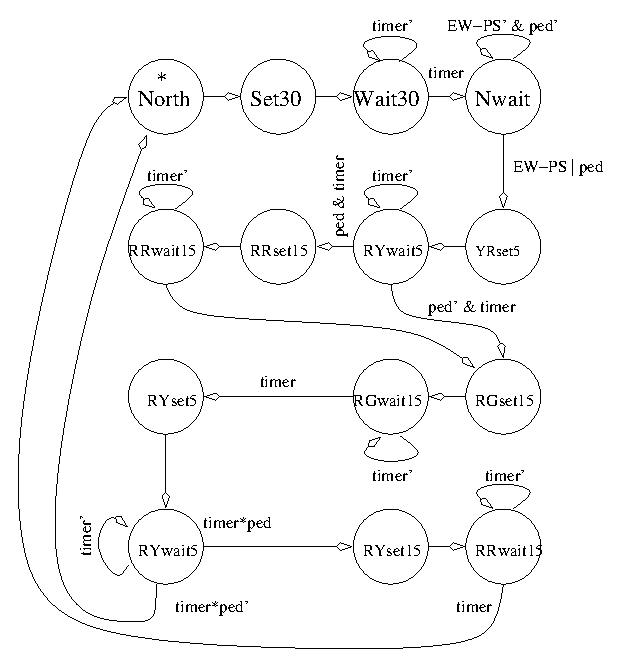
\includegraphics{Sol7-13}}
                    \caption{The FSM for a traffic light controller.}
                \end{figure}

                \begin{tabular}{|l|||l|l|l|} \hline
                    \multicolumn{4}{|c|}{outputs from the digital circuit}    \\ \hline \hline
                    state & Timer     & NS light  & EWlight     \\ \hline
                    & 00 down   & 00 red    & 00 red      \\ \hline
                    & 01 5 sec  & 01 red    & 01 red      \\ \hline
                    & 10 15 sec & 10 yellow & 10 yellow   \\ \hline
                    & 11 30 sec & 11 green  & 11 green    \\ \hline \hline
                    North    & 00       & 11          & 00  \\ \hline
                    set30 & 11       & 11          & 00  \\ \hline
                    wait30& 00       & 11          & 00  \\ \hline
                    Nwait    & 00       & 11          & 00  \\ \hline

                    YRset5  & 01       & 10          & 00  \\ \hline
                    YRwait5 & 00       & 10          & 00  \\ \hline

                    RRset15 & 10       & 00          & 00  \\ \hline
                    RRwait15& 00       & 00          & 00  \\ \hline

                    RGset15 & 10       & 00          & 11  \\ \hline
                    RGwait15& 00       & 00          & 11  \\ \hline
                \end{tabular}

                The memory input equations are a snap.
                \begin{description}
                    \item $D_{North} = Q_{RYwait5}*ped*timer + Q_{RRwait15}*timer $
                    \item $D_{Set30} = Q_{North} $
                    \item $D_{Wait30} = Q_{Set30} + Q_{Wait30}*timer' $
                    \item $D_{Nwait} = Q_{Wait30}*timer + Nwait*EW_PS'*ped' $
                    \item $D_{YRset5} = Q_{Nwait}*(EW_PS + ped) $
                    \item $D_{YRwait5} = Q_{YRset5} +Q_{YRwait5}*timer' $
                    \item $D_{RRset15} = Q_{YRwait5}*ped*timer $
                    \item $D_{RRwait15} = Q_{RRset15} + Q_{RRwait15}*timer' $
                    \item $D_{RGset15} = Q_{YRwait5}*ped'*timer + Q_{RRwait15}*timer $
                    \item $D_{RGwait15} = Q_{RGset15} $
                    \item $D_{RYset5} = Q_{RGwait15}*timer' $
                    \item $D_{RYwait5} = Q_{RYset5} + Q_{RYwait5}*timer' $
                    \item $D_{RRset15} = Q_{RYwait5}*ped $
                    \item $D_{RRwait15} = Q_{RRset15} +Q_{RRwait15}*timer' $
                \end{description}

                The output equations
                \begin{description}
                    \item $Z_{t1}  = Q_{set30} + Q_{RRset15} $
                    \item $Z_{t0}  = Q_{set30} + Q_{YRset5} $
                    \item $Z_{ns1} = Q_{North} + Q_{set30} + Q_{wait30} + Q_{Nwait} +Q_{YRset5}+Q_{YRwait5} $
                    \item $Z_{ns0} = Q_{North} + Q_{set30} + Q_{wait30} + Q_{Nwait} $
                    \item $Z_{ew1} = Q_{RGset15} + Q_{RGwait15} $
                    \item $Z_{ew0} = Q_{RGset15} + Q_{RGwait15} $
                \end{description}
            }
        \end{onlysolution}
\end{enumerate}
